\section{Fluctuations}

We now want to study the path integral going beyond the saddle-point approximation and understand the impact of fluctuations. We start from the LG partition function\TODO{Add reference to Kardar book (Ch. 3) and the notes statistical field theory by D. Tong.}
\[
    \mathcal{Z} = \int \mathcal{D}m(\mathbf{x}) e^{-\int \mathrm{d}^d \mathbf{x} \left[ \frac{t}{2}m^2(\mathbf{x}) + u m^4(\mathbf{x}) + \frac{\kappa}{2}(\nabla m)^2 \right]}.
\]
We have already saw that the saddle-point approximation to this partition function gives a good description of the phase transition, and allows us to compute the critical exponents. However, it is not clear whether the saddle-point approximation is reliable, and whether the critical exponents obtained from it are correct. To answer these questions, we need to study the fluctuations around the saddle-point solution.

For \( u > 0 \) and without imposing fixed boundary conditions, we saw that the saddle-point solution corresponds to
\[
    m(\mathbf{x}) \equiv \overline{m} = \begin{dcases}
        0                    & t > 0, \\
        \sqrt{\frac{-t}{4u}} & t < 0.
    \end{dcases}
\]

Since we want to examine the fluctuations around the saddle-point solution, we write the field \( m(\mathbf{x}) \) as the sum of the saddle-point solution \( \overline{m} \) and a fluctuation field \( \phi(\mathbf{x}) \):
\[
    m(\mathbf{x}) = \overline{m} + \phi(\mathbf{x}).
\]
Substituting this expression into the LG free energy, we can expand to the 2nd order in \( \phi(\mathbf{x}) \) the powers of \(m(\mathbf{x})\) and its derivatives, to obtain
\[
    \begin{dcases}
        (\nabla m)^2 = (\nabla\phi(\mathbf{x}))^2,                                          \\
        m^2          = \overline{m}^2 + 2\overline{m}\phi(\mathbf{x}) + \phi(\mathbf{x})^2, \\
        m^4          = \overline{m}^4 + 4\overline{m}^3\phi(\mathbf{x}) + 6\overline{m}^2\phi^2(\mathbf{x}) + \mathcal{O}(\phi(\mathbf{x})^3).
    \end{dcases}
\]
Therefore, substituting these expressions back into the free energy, we have
\[
    \begin{aligned}
        F_{LG} & \simeq V \left( \frac{t}{2}\overline{m}^2 + u\overline{m}^4 \right) + \int \mathrm{d}^d \mathbf{x} \left[ \frac{\kappa}{2}(\nabla\phi)^2 + \frac{t + 12u\overline{m}^2}{2}\phi^2 \right] \\
               & \simeq F[\overline{m}] + \int \mathrm{d}^d \mathbf{x} \left[ c_1 \phi^2(\mathbf{x}) + c_2(\nabla\phi)^2 \right],
    \end{aligned}
\]
where \(V = \int \mathrm{d}^d \mathbf{x} \) is just the volume of the system, and we have defined \(c_1(t)\) and \(c_2\) as follows:
\[
    c_1(t) = \frac{t + 12u\overline{m}^2}{2} > 0, \quad c_2 = \frac{\kappa}{2} > 0.
\]
Note that there are no linear terms in \( \phi \), which follows from the fact that we are expanding around the minimum of the free energy (where \( \tfrac{\partial F}{\partial m} = 0 \)).

Since we have defined \(m(\mathbf{x}) = \overline{m} + \phi(\mathbf{x})\), we can perform the functional integral over \( \phi(\mathbf{x}) \)
\[
    \mathcal{D} m(\mathbf{x}) \mapsto \mathcal{D}\phi(\mathbf{x}),
\]
to compute the partition function, and thus the free energy. This will allow us to understand how fluctuations modify the critical behavior of the system with respect to the saddle-point prediction.

In order to rewrite the free energy in a more convenient form, let us remember that in general
\[
    \mathcal{Z} = \int \mathcal{D} m(\mathbf{x}) e^{-F[m(\mathbf{x})]},
\]
which is a functional integral over all possible field configurations \( m(\mathbf{x}) \). We have moved onto an integration over the fluctuations \( \phi(\mathbf{x}) \), and now it is useful to consider the Fourier transform of the field \( \phi(\mathbf{x}) \) with the idea of diagonalizing the free energy in momentum space:
\[
    \phi_{\mathbf{q}} = \int \mathrm{d}^d \mathbf{x} \, e^{-i\mathbf{q} \cdot \mathbf{x}} \phi(\mathbf{x}) \implies \phi(\mathbf{x}) = \int \frac{\mathrm{d}^d \mathbf{q}}{(2\pi)^d} \, e^{i\mathbf{q} \cdot \mathbf{x}} \phi_{\mathbf{q}},
\]
where \( \phi(\mathbf{x}) \in \mathbb{R} \) has to remain a real field, so that we need to impose \( \phi_{\mathbf{q}}^* = \phi_{-\mathbf{q}} \), and \( \mathbf{q} \) are the momenta of the field. Remember that \( \phi(\mathbf{x}) \) was obtained by \textbf{coarse-graining}\footnote{With \textit{coarse-graining} we mean the process of averaging over short-distance fluctuations, which is exactely what we have been doing in the Landau-Ginzburg theory to obtain a mesoscopic description of the system.} a microscopic spin configuration (we derived in this way \(m(\mathbf{x})\) and \(\phi(\mathbf{x})\) are the fluctuations around the mean field \(\overline{m}\), so they have the same nature). Therefore, we can assume that \( \phi(\mathbf{x}) \) does not vary over length scales that are smaller than the spin-spin distance \( a \) (the lattice spacing). In turn, it means we can introduce a cutoff \( \Lambda \) in momentum space, and require
\[
    \phi_{\mathbf{q}} = 0 \text{ if } |\mathbf{q}| > \Lambda = 1/a.
\]
Indeed, if the field \( \phi(\mathbf{x}) \) does not vary over length scales smaller than \( a \), then its Fourier transform \( \phi_{\mathbf{q}} \) must vanish for momenta larger than \( 1/a \), since such momenta must correspond to fluctuations that vary on length scales smaller than \( a \). Therefore, if \( \phi(\mathbf{x}) \) is smooth and does not have any sharp features on length scales smaller than \( a \), then its Fourier transform \( \phi_{\mathbf{q}} \) must be concentrated around low momenta, and must vanish for momenta larger than \( 1/a \).

Next, if we we plug the Fourier transform into the free energy, we can effectively diagonalize it in momentum space. In fact, we have
\[
    F_{LG} - F[\overline{m}] = \int \frac{\mathrm{d}^d \mathbf{q}_1}{(2\pi)^d} \int \frac{\mathrm{d}^d \mathbf{q}_2}{(2\pi)^d} \int \mathrm{d}^d \mathbf{x} \left( -c_2 \mathbf{q}_1 \cdot \mathbf{q}_2 + c_1 \right) \phi_{\mathbf{q}_1} \phi_{\mathbf{q}_2} e^{i(\mathbf{q}_1 + \mathbf{q}_2) \cdot \mathbf{x}},
\]
where now we have two integrations in momentum space (since the field \(\phi(\mathbf{x})\) appeared always squared), and one integration in real space. Using the definition of the Dirac delta function
\[
    \int \mathrm{d}^d \mathbf{x} \, e^{i(\mathbf{q}_1 + \mathbf{q}_2) \cdot \mathbf{x}} = (2\pi)^d \delta^d(\mathbf{q}_1 + \mathbf{q}_2),
\]
we can perform the integration in real space to enforce the constraint \( \mathbf{q} = \mathbf{q}_1 = -\mathbf{q}_2 \), and we finally arrive at
\[
    F_{LG} - F[\overline{m}] = \int \frac{\mathrm{d}^d \mathbf{q}}{(2\pi)^d} (c_2 q^2 + c_1) \phi_{\mathbf{q}} \phi_{-\mathbf{q}} = \int \frac{\mathrm{d}^d \mathbf{q}}{(2\pi)^d} (c_2 q^2 + c_1) |\phi_{\mathbf{q}}|^2,
\]
since \(\phi_{\mathbf{q}} \phi_{-\mathbf{q}} = \phi_{\mathbf{k}} \phi_{\mathbf{k}}^* = |\phi_{\mathbf{q}}|^2\) is the definition of the squared modulus of a complex number. We have thus succeeded in diagonalizing the free energy in momentum space and we can now perform explicitly the functional integral to compute the partition function.

To compute explicitly the partition function, we need to change variables in the original functional path-integral in order to express it in terms of the Fourier modes \( \phi_{\mathbf{q}} \). We have
\[
    \int \mathcal{D}\phi(\mathbf{x}) \propto \int \mathcal{D}\phi_{\mathbf{q}} = \prod_{\mathbf{q}} \int \mathrm{d}\phi_{\mathbf{q}}, \qquad (*)
\]
where we need to impose the additional reality constraint \( \phi_{\mathbf{q}}^* = \phi_{-\mathbf{q}} \). Finally, we get
\[
    \mathcal{Z} = \left( \prod_{\mathbf{q}} \int \mathrm{d}\phi_{\mathbf{q}} \right) e^{- \int \frac{\mathrm{d}^d \mathbf{q}}{(2\pi)^d} (c_2 q^2 + c_1) |\phi_{\mathbf{q}}|^2},
\]
where we neglected possible overall normalization constants, which may appear as the Jacobian of the change of variable \((*)\). At this point, it is useful to adopt a further simplification and imagine that we are working in a finite volume \( V = L^d \), such that the integral over \( \mathbf{q} \) is then replaced by a sum over the quantized momenta \( \mathbf{q} = \frac{2\pi}{L} \mathbf{n} \), with \(\mathbf{n} \in \mathbb{Z}^d \):
\[
    \int \frac{\mathrm{d}^d \mathbf{q}}{(2\pi)^d} (\cdots) \longrightarrow \frac{1}{V} \sum_{\mathbf{q}} (\cdots),
\]
which in some way is equivalent to a sort of spatial cutoff. Making this substitution we arrive at
\[
    \mathcal{Z} = \prod_{\mathbf{q}}' \left[ \int \mathrm{d}\phi_{\mathbf{q}} \, e^{- \frac{1}{V} (c_2 q^2 + c_1) |\phi_{\mathbf{q}}|^2} \right]
\]
Here, \( \prod\limits_{\mathbf{q}}' \) means that we are taking the product over \( \mathbf{q} = (q_1, \dots, q_d) \) such that \( q_1 > 0 \).
Since the original real-space field is real-valued, its Fourier components are constrained by \(\phi_{-\mathbf{q}} = \phi_{\mathbf{q}}^*\), which implies that \(\phi_{\mathbf{q}}\) and \(\phi_{-\mathbf{q}}\) are not independent degrees of freedom. To avoid double-counting when computing the partition function, the product must be restricted to half of the momentum space, which is denoted by the primed product \(\prod_{\mathbf{q}}'\) (e.g., considering only \(q_1 > 0\), choice which allows us to consider only positive frequencies). Furthermore, because the integrand depends only on \(q^2\) and \(|\phi_{\mathbf{q}}|^2\), it is entirely symmetric under the exchange \(\mathbf{q} \to -\mathbf{q}\). Therefore, evaluating the product over the restricted half-space is mathematically equivalent to taking the square root of the product over the entire momentum space:
\[
    \prod_{\mathbf{q}}' \left[ \dots \right] = \sqrt{\prod_{\mathbf{q}} \left[ \dots \right]}.
\]

So finally we can use these results to rewrite the partition function as
\[
    \mathcal{Z} = \sqrt{\prod_{\mathbf{q}} \left[ \int \mathrm{d}\phi_{\mathbf{q}} \, e^{- \frac{1}{V} (c_2 q^2 + c_1) |\phi_{\mathbf{q}}|^2} \right]},
\]
which is now an easy product of decoupled gaussian integrals over complex variables. Using
\[
    \int_{\mathbb{C}} \mathrm{d}z \, e^{-|z|^2 / a} = \int\limits_{-\infty}^{+\infty} \int\limits_{-\infty}^{+\infty} \mathrm{d}x \mathrm{d}y \, e^{-(x^2 + y^2) / a} = \pi a,
\]
we arrive at the final expression for the partition function
\[
    \mathcal{Z} = \prod_{\mathbf{q}} \sqrt{\frac{\pi V}{c_2 q^2 + c_1}}.
\]
Therefore, neglecting irrelevant overall constants and using
\[
    \frac{1}{V} \log \left( \prod_{\mathbf{q}} (\dots) \right) = \frac{1}{V} \sum_{\mathbf{q}} \log(\dots) \simeq \int \frac{\mathrm{d}^d \mathbf{q}}{(2\pi)^d} \log(\dots),
\]
we can rewrite
\[
    \boxed{ \frac{F_{LG} - F[\overline{m}]}{V} = - \frac{1}{2} \int \frac{\mathrm{d}^d \mathbf{q}}{(2\pi)^d} \log \left( \frac{1}{c_2 q^2 + c_1} \right) },
\]

which is the contribution to the free energy coming from the fluctuations around the saddle-point solution. Equivalently, we can write the total free energy as
\[
    F_{LG} = V \left( \frac{t}{2}\overline{m}^2 + u\overline{m}^4 \right) + \frac{V}{2} \int \frac{\mathrm{d}^d \mathbf{q}}{(2\pi)^d} \log(c_2 q^2 + c_1).
\]
The contribution we found is non-trivial, and it modifies the critical behavior of the system with respect to the mean-field (or, more generally, the SPA) prediction. In particular, it can lead to a divergence of the heat capacity at the critical temperature \( T_c \), which is a signature of a second-order phase transition, but we will see this more explicitly in the next section.

\subsection{Heat Capacity}

We will now use the previous form of the free energy to compute the heat capacity close to the critical temperature \( T_c \). Comparing the saddle-point prediction with the fluctuation contribution will allow us to identify the upper critical dimension for the Ising model: when \( d > D_c \) is above the upper critical dimension, the saddle-point approximation is reliable and the critical exponents are given by the mean-field predictions. Instead, when \( d < D_c \) is below the upper critical dimension, fluctuations become important and modify the critical exponents with respect to their mean-field values.

Remember that we defined the \textbf{heat capacity} by the second derivative of the free energy with respect to the temperature \( T \):
\[
    C = -T \frac{\partial^2}{\partial T^2} F.
\]
Recall we identified the parameter \( t \) in the LG free energy by
\[
    t = a(T - T_c) + \mathcal{O}((T - T_c)^2),
\]
since we needed \( t \) to vanish at the critical temperature \( T_c \) and change sign across the transition. Therefore, we can express the heat capacity in terms of derivatives with respect to \( t \), which at the leading order, relates to derivatives with respect to \( T \) as
\[
    \frac{\partial}{\partial T} = a \frac{\partial}{\partial t}.
\]
We can thus rewrite the heat capacity as
\[
    C \simeq T a^2 \frac{\partial^2}{\partial t^2} \left[ \frac{1}{\beta} \log \mathcal{Z} \right] \simeq T_c a^2 \frac{\partial^2}{\partial t^2} \left[ T_c \log \mathcal{Z}(t) \right].
\]

The idea is now to compute the heat capacity using the partition function obtained by including the fluctuations, and compare it with the saddle-point prediction. This will allow us to understand whether the saddle-point approximation is reliable, and whether the critical exponents obtained from it are correct.

\begin{itemize}
    \item First, let us recall the \textbf{saddle-point approximation} for \( \mathcal{Z}_{LG} \) at \( h=0 \), given by
          \[
              \overline{m} = \begin{dcases}
                  0                    & t > 0, \\
                  \sqrt{\frac{-t}{4u}} & t < 0,
              \end{dcases}
          \]
          which was derived in the previous section. Substituting this solution into the LG free energy,
          \[
              \log \mathcal{Z}_{LG} \simeq -V \left( \frac{t}{2}\overline{m}^2 + u \overline{m}^4 \right) = \begin{dcases}
                  0                  & \text{for } t > 0, \\
                  +V \frac{t^2}{16u} & \text{for } t < 0,
              \end{dcases}
          \]
          \[
              \Rightarrow \quad C = \begin{dcases}
                  C_0                            & \text{for } t > 0, \\
                  C_0 + V a^2 T_c^2 \frac{1}{8u} & \text{for } t < 0.
              \end{dcases}
          \]
          Here \( C_0 \) is a constant which comes from the regular part of the partition function (namely, \( \log \mathcal{Z} = \log \mathcal{Z}_0 + \log \mathcal{Z}_{LG} \), where \( \log \mathcal{Z}_0 \) contains all the \( m \)-independent terms that we neglected in the LG free energy, since they do not contribute to the critical behavior).

          Therefore, the saddle-point (or mean-field) prediction is
          \begin{figure}[H]
              \begin{minipage}{0.6\textwidth}
                  \centering
                  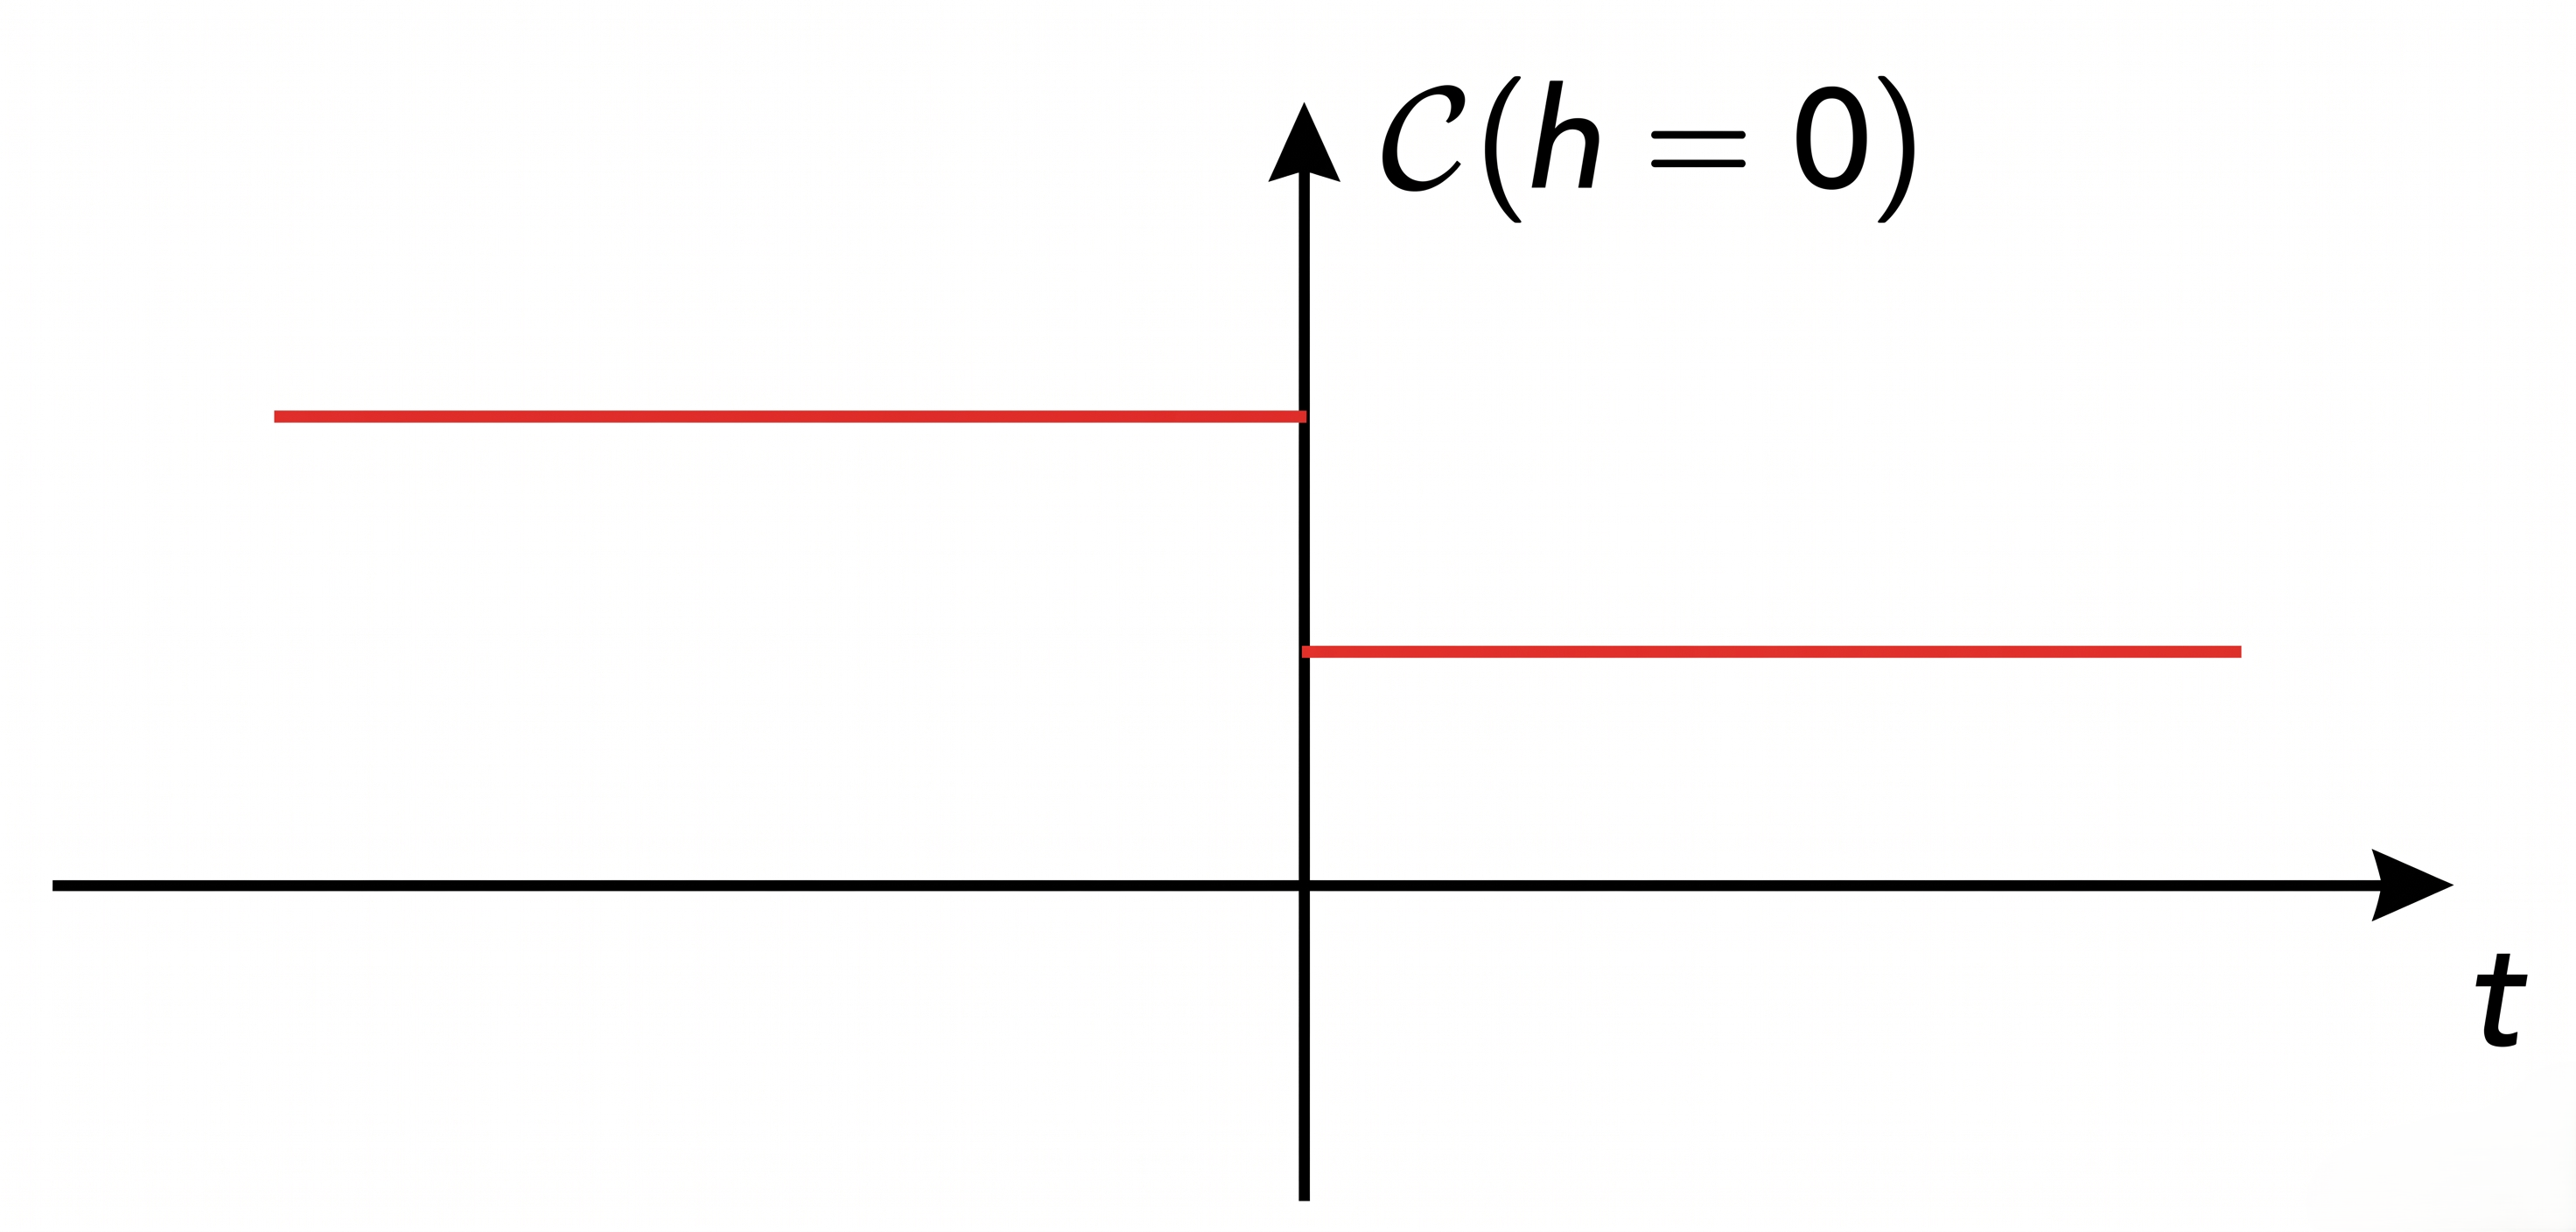
\includegraphics[width=0.8\textwidth]{img/fluctuations_C.png}
              \end{minipage}
              \hfill
              \begin{minipage}{0.35\textwidth}
                  \caption{Plot of the heat capacity in absence of external field \( C(h=0) \) versus reduced temperature \( t \), showing a step discontinuity at \( t=0 \) according to the mean-field approximation.}
              \end{minipage}
          \end{figure}
          Recall that the \( \alpha \)-exponent is defined by
          \[
              C_\pm(t(T), h=0) \sim A_\pm |t|^{-\alpha},
          \]
          since it describes the divergence of the heat capacity at the critical temperature \( T_c \). The saddle-point approximation predicts \( \alpha = 0 \): we do not have an expression depending on \( t \) in the heat capacity, but just a step discontinuity at \( t=0 \).

    \item Next, let us compute how the prediction is modified using the partition function obtained by including the \textbf{fluctuations} up to second order, where again we now include the regular part \( \mathcal{Z}_0 \) of the partition function, the saddle-point contribution, and the fluctuation contribution:
          \[
              \log \mathcal{Z} = \log \mathcal{Z}_0 - V\left( \frac{t}{2}\overline{m}^2 + u \overline{m}^4 \right) - \frac{V}{2} \int \frac{\mathrm{d}^d \mathbf{q}}{(2\pi)^d} \log(c_2 q^2 + c_1),
          \]
          where we had
          \[
              c_2 = \frac{\kappa}{2} \quad \text{and} \quad c_1 = \frac{t + 12u\overline{m}^2}{2} = \begin{dcases}
                  \frac{t}{2} & \text{for } t > 0, \\
                  -t          & \text{for } t < 0,
              \end{dcases}
          \]
          recalling the SPA solution for \( \overline{m}(t) \).
          Therefore, the new contribution to the heat capacity is given by the second derivative with respect to \( t \) of the fluctuation contribution to the free energy:
          \[
              -\frac{V}{2} \frac{\partial^2}{\partial t^2} \int \frac{\mathrm{d}^d \mathbf{q}}{(2\pi)^d} \log(c_2 q^2 + c_1) = \begin{dcases}
                  \frac{V}{2} \int \frac{\mathrm{d}^d \mathbf{q}}{(2\pi)^d} \frac{1}{(\kappa q^2 + t)^2} & \text{for } t > 0, \\
                  2V \int \frac{\mathrm{d}^d \mathbf{q}}{(2\pi)^d} \frac{1}{(\kappa q^2 - 2t)^2}         & \text{for } t < 0.
              \end{dcases}
          \]
          If we now (after some algebra and dimensional analysis) introduce the following length scale
          \[
              \xi^{-2} = \begin{dcases}
                  \frac{t}{\kappa}   & \text{for } t > 0, \\
                  -\frac{2t}{\kappa} & \text{for } t < 0,
              \end{dcases}
          \]
          we can rewrite the previous expression as
          \[
              -\frac{V}{2} \frac{\partial^2}{\partial t^2} \int \frac{\mathrm{d}^d \mathbf{q}}{(2\pi)^d} \log(c_2 q^2 + c_1) \sim \frac{1}{\kappa^2} \int \frac{\mathrm{d}^d \mathbf{q}}{(2\pi)^d} \frac{1}{(q^2 + \xi^{-2})^2}
          \]
          where we did not keep track of the numerical prefactors. We now have to explicit some considerations from dimensional analysis:
          \begin{itemize}
              \item The integral now has dimension \(\sim L^{4-d}\). In fact, the integration measure \(\mathrm{d}^d \mathbf{q}\) has dimension \(\sim L^{-d}\), while the integrand has dimension \(\sim L^4\) (since \(q^2\) and \(\xi^{-2}\) have dimension \(\sim L^{-2}\)).
              \item For \(d \geq 4\) the integral diverges at large \(q\) (going to zero), and is dominated by the momentum cutoff \(\Lambda\): we would have an integrand behaving as \(q^{-4}\) at large \(q\), and thus the integral would behave as \(\Lambda^{d-4}\).
              \item For \(d < 4\) the integral is convergent. It can be made dimensionless by rescaling \(q \mapsto q' = q \xi^{-1}\), since we saw that in the momentum space \([q_i] \sim L^{-1}\) (keeping in mind the example of spherical coordinates, where \(\mathrm{d} \mathbf{q} = q^{d-1} \, \mathrm{d} q\, \mathrm{d} \Omega\)). After the rescaling, the integral becomes
                    \[
                        \xi^{4-d}\int \frac{\mathrm{d}^d \textbf{q}'}{(2\pi)^d} \frac{1}{(q'^2 + 1)^2},
                    \]
                    which is now dimensionless and convergent. Therefore, the original integral behaves asymptotically as \(\xi^{4-d}\) for \(d < 4\).
          \end{itemize}
          Therefore we have:
          \[
              -\frac{\partial^2}{\partial t^2} \frac{V}{2} \int \frac{\mathrm{d}^d \mathbf{q}}{(2\pi)^d} \log(c_2 q^2 + c_1) \sim \frac{1}{\kappa^2} \begin{dcases}
                  \Lambda^{d-4} & \text{for } d \geq 4, \\
                  \xi^{4-d}     & \text{for } d < 4,
              \end{dcases}
          \]
          which is the asymptotic behavior of the fluctuation contribution to the heat capacity (when \(d = 4\), the divergence in \(\Lambda\) is logarithmic).

          We obtained that in \(d \geq 4\) fluctuation corrections to the heat capacity add a constant term to the heat capacity for both \( t > 0 \) and \( t < 0 \). Instead, for \( d < 4 \), the divergence \( \xi \sim t^{-1/2} \) at the transition leads to a divergence of the heat capacity with a critical exponent
          \[
              \alpha = \frac{4 - d}{2}
          \]
\end{itemize}

\begin{figure}[H]
    \centering
    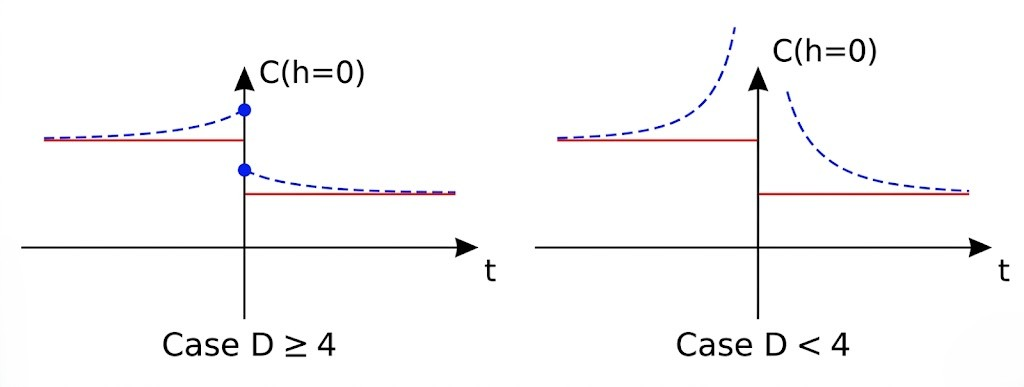
\includegraphics[width=0.8\textwidth]{img/fluctuations_C_comparison.jpg}
    \caption{Two side-by-side plots showing the heat capacity \( C(h=0) \) versus reduced temperature \( t \). The left plot illustrates the case \( d \geq 4 \) with a constant fluctuation correction, while the right plot illustrates the case \( d < 4 \) where the heat capacity diverges at \( t=0 \).}
\end{figure}

The exponent \( \alpha = \frac{4 - d}{2} \) is not exact because it only takes into account quadratic fluctuations. However, the fact that \( C \) diverges for \( d < 4 \) means that the saddle-point conclusions are not reliable for \( d < 4 \), identifying \( d = 4 = D_c \) as the upper critical dimension.

\subsection{Correlation Functions}

The same machinery can be used to compute \uline{correlation functions} and in particular the \textbf{connected correlator}
\[
    G^c(\mathbf{x}, \mathbf{y}) = \langle (m(\mathbf{x}) - \overline{m})(m(\mathbf{y}) - \overline{m}) \rangle = \langle \phi(\mathbf{x}) \phi(\mathbf{y}) \rangle,
\]
where \( \langle \dots \rangle \) denotes the ensemble average. The computation is not hard but we will not see it explicitly, giving only the final result, which reads
\[
    G^c(\mathbf{x}, \mathbf{y}) = - \frac{1}{\kappa} I_d(\mathbf{x} - \mathbf{y}),
\]
where
\[
    I_d(\mathbf{x}) = - \int \frac{\mathrm{d}^d \mathbf{q}}{(2\pi)^d} \frac{e^{i \mathbf{q} \cdot \mathbf{x}}}{q^2 + \xi^{-2}},
\]
and \( \xi \) is the length scale introduce above
\[
    \xi^{-2} = \begin{dcases}
        \frac{t}{\kappa}   & \text{for } t > 0, \\
        -\frac{2t}{\kappa} & \text{for } t < 0.
    \end{dcases}
\]
One can study this function and infer the following behavior
\[
    I_d(\mathbf{x}) \sim \begin{dcases}
        \frac{1}{|\mathbf{x}|^{d-2}}               & |\mathbf{x}| \ll \xi, \\
        \frac{e^{-|\mathbf{x}|/\xi}}{|\mathbf{x}|} & |\mathbf{x}| \gg \xi.
    \end{dcases}
\]
For \( t \neq 0 \), \( \xi \) is naturally interpreted as a spatial correlation length. When \( t \to 0 \), we have consequently \( \xi \to \infty \), such that the connected correlators decay as a power law.

\subsection{The Ginzburg Criterion}

Before moving on, we complete our discussion of LG theory with the Ginzburg criterion. Recall our predictions for the heat capacity using the quadratic corrections to the saddle point for \( d < 4 \)

\begin{figure}[H]
    \begin{minipage}{0.6\textwidth}
        \centering
        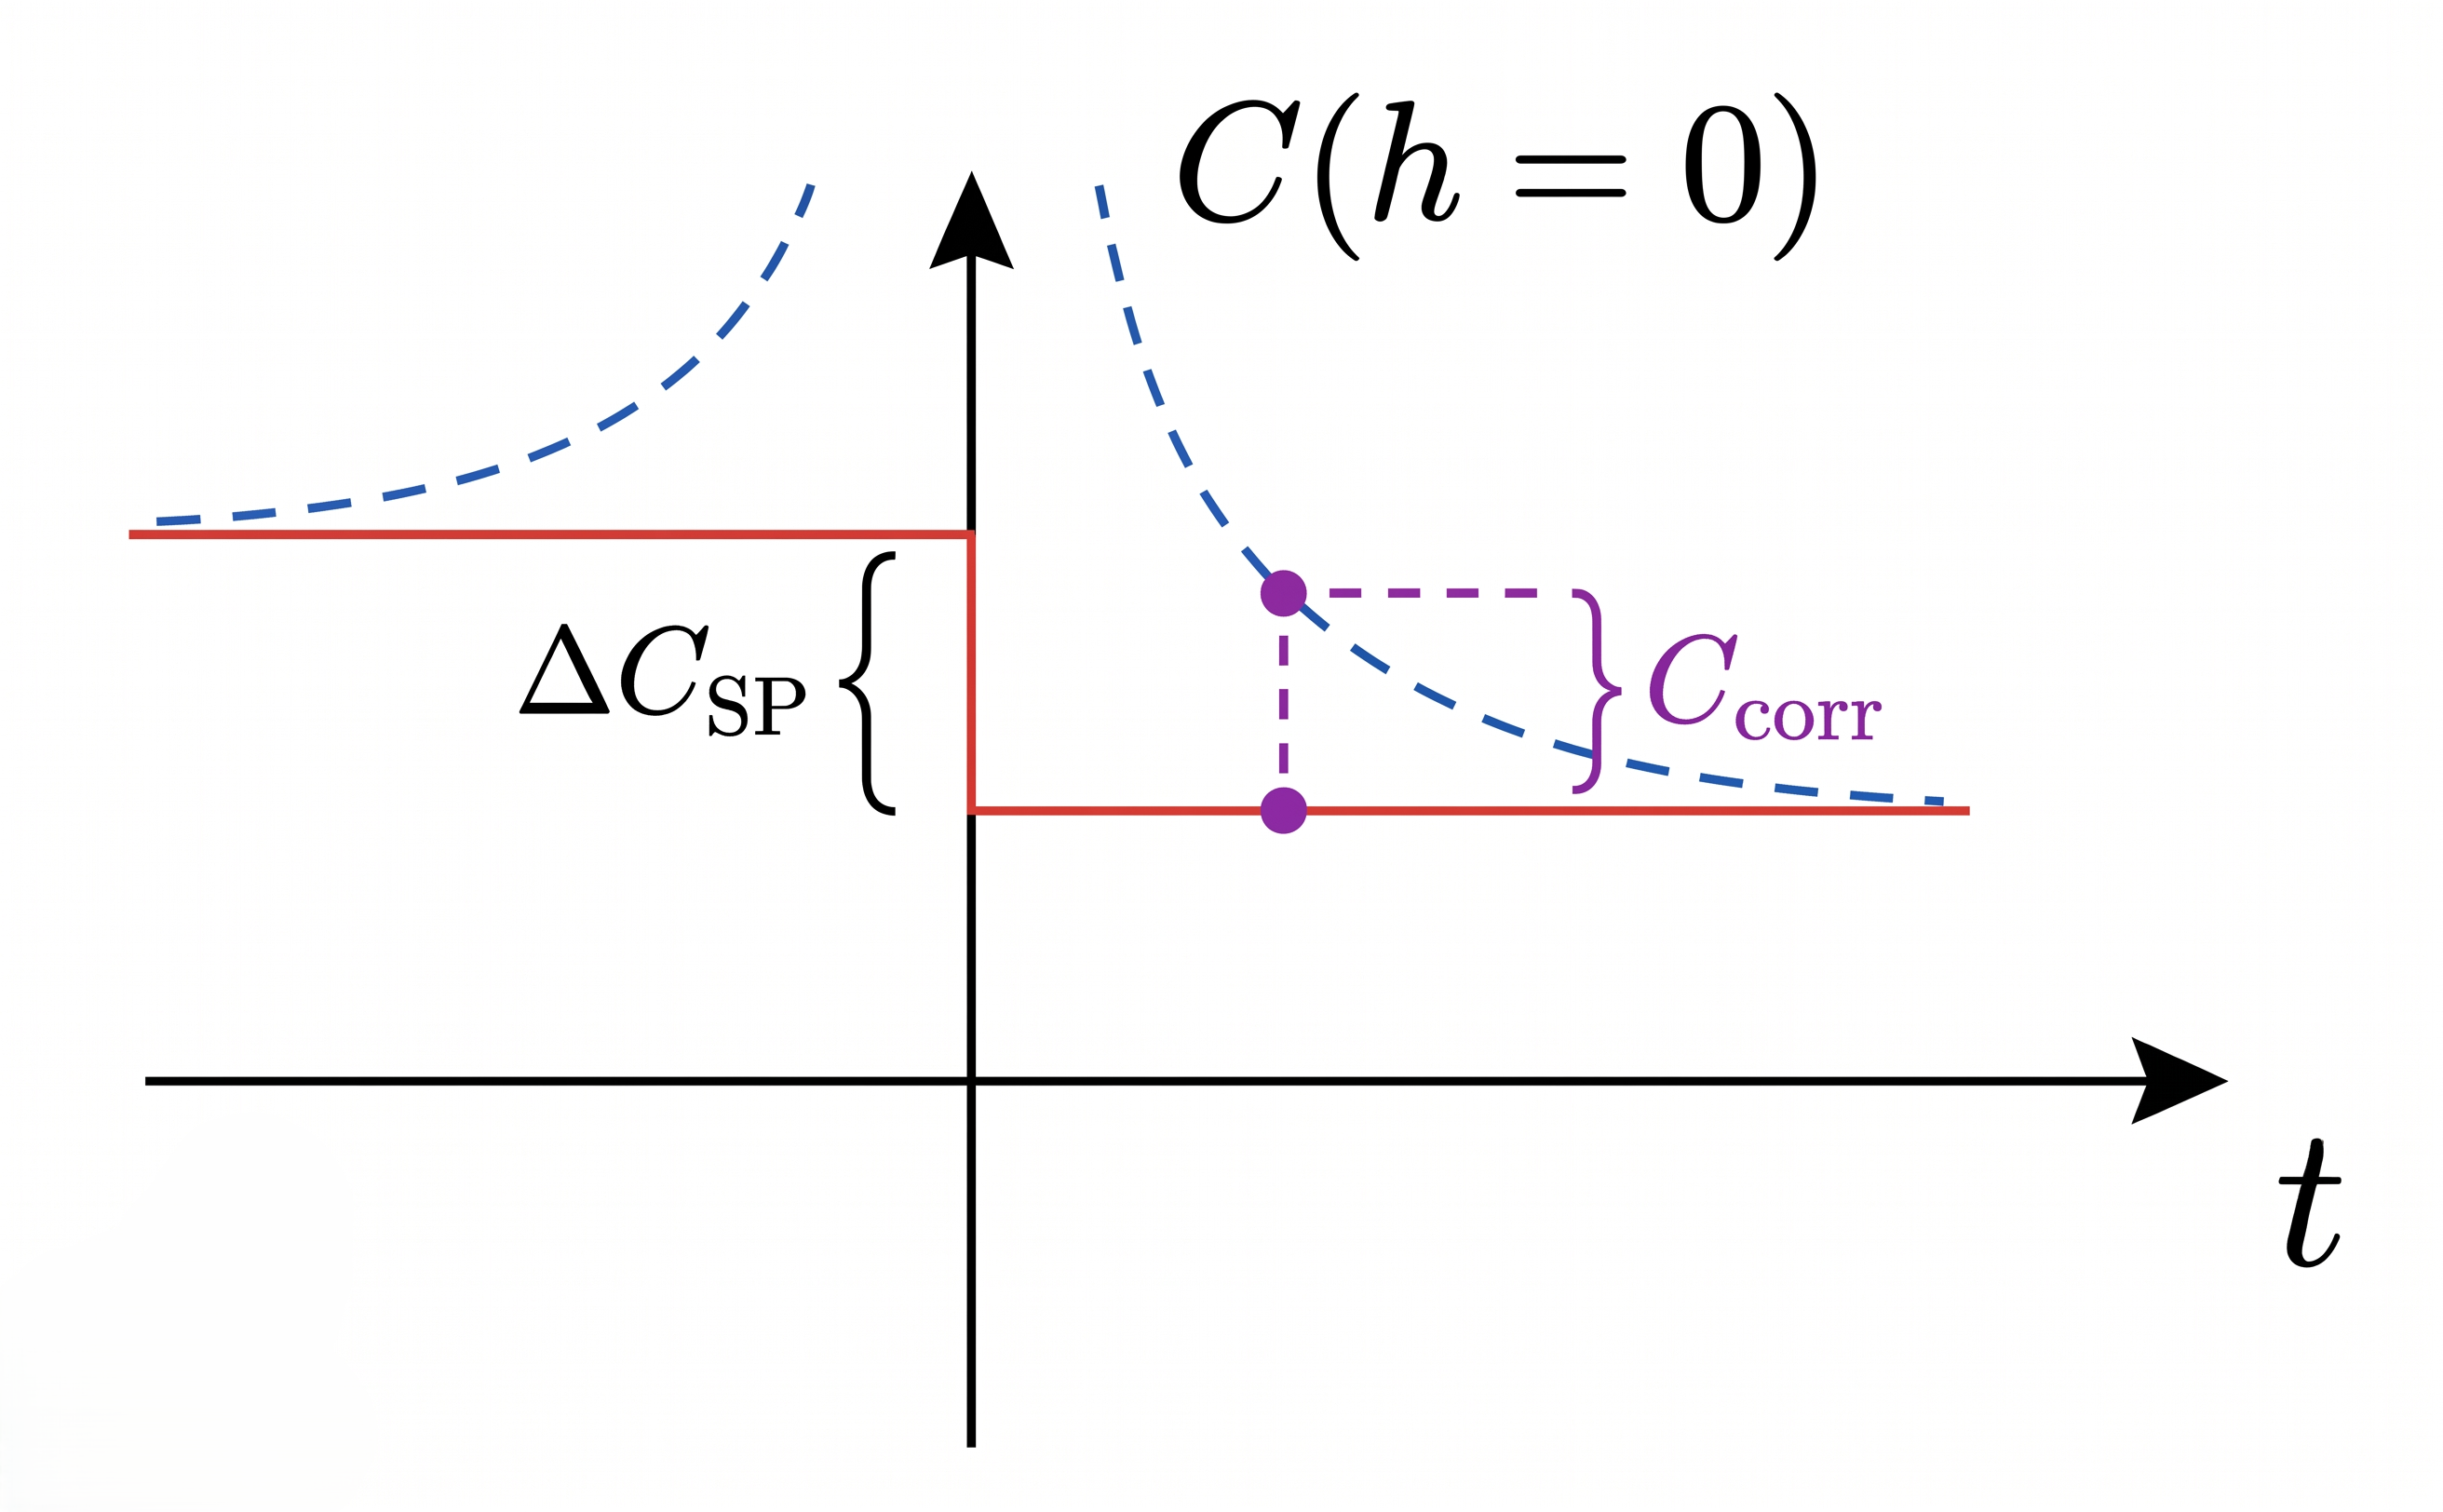
\includegraphics[width=0.8\textwidth]{img/fluctuations_ginzburg_crit_C.png}
    \end{minipage}
    \hfill
    \begin{minipage}{0.35\textwidth}
        \caption{Plot of the heat capacity \( C(h=0) \) versus reduced temperature \( t \), showing the mean-field step \( \Delta C_{SP} \) and the fluctuation correction \( C_{corr} \) diverging at \( t=0 \).}
    \end{minipage}
\end{figure}

Denote by \( C_{corr} \) the difference between the calculated value and the SP predictions. Further, denote by \( \Delta C_{SP} \) the value of ``the jump'' of the heat capacity predicted by the saddle-point approximation. We can estimate the importance of fluctuations by comparing \( C_{corr} \) with \( \Delta C_{SP} \), with the idea to find a regime where fluctuations are negligible and the saddle-point approximation is reliable.

Fluctuations are important if their contribution to the heat capacity is larger than the jump predicted by the saddle-point approximation, which alternatively reads \(C_{corr} \gg \Delta C_{SP}\); we thus expect to obtain correct results from the saddle-point approximation when
\[
    C_{corr} \ll \Delta C_{SP}.
\]
Recalling that, for \( d \leq 4 \), we have found a contribution to the heat capacity from fluctuations which behaves as
\[
    C_{corr} \sim \frac{1}{\kappa^2} \xi^{4-d} \sim \frac{1}{\kappa^2} |t|^{-\frac{4-d}{2}},
\]
where we used the definition of the length scale \( \xi \) introduced above (without considering numerical factors depending on the sign of \( t \)). On the other hand, the jump predicted by the saddle-point approximation, as we computed, is proportional to \(\tfrac{1}{u}\).

Therefore, the condition \( C_{corr} \ll \Delta C_{SP} \) can be rewritten as
\[
    \implies \quad |t|^{\frac{d-4}{2}} \ll \frac{\kappa^2}{u} \qquad \Rightarrow \qquad |t| \gg t_G \simeq \left( \frac{u}{\kappa^2} \right)^{\frac{2}{4-d}}.
\]
This is Ginzburg's criterion. We see that, as we expected, for \( |t| \) sufficiently low the fluctuations are important. However, it gives a temperature \( t_G \) above which fluctuations become less important, thus the saddle-point approximation becomes reliable in that regime. In some experiments we may not get below \( t_G \), so we may see a critical behaviour which is similar to the mean-field result. This is just an artifact due to the fact that we are not sufficiently close to \( T_c \), and thus we are not able to see the true critical behavior of the system.